% !TeX root = ../main/main.tex
\documentclass[../main/main.tex]{subfiles}

\begin{document}
\espacio
  En este capítulo se muestran los conceptos referentes al entorno de virtualización de contenedores Docker, definición y proceso de la minería de criptomonedas y ataques tipo zombie.

  \section{Antecedentes}

  La minería de criptomonedas se convirtió en un negocio rentable para los cibercriminales desde el surgimiento de la técnica de minería en exploradores web, misma que se aprovecha del cómputo de los clientes en un sin número de sitios web.

  \begin{figure}[H]
    \centering
    \caption{Geografía de la minería de criptomonedas}
    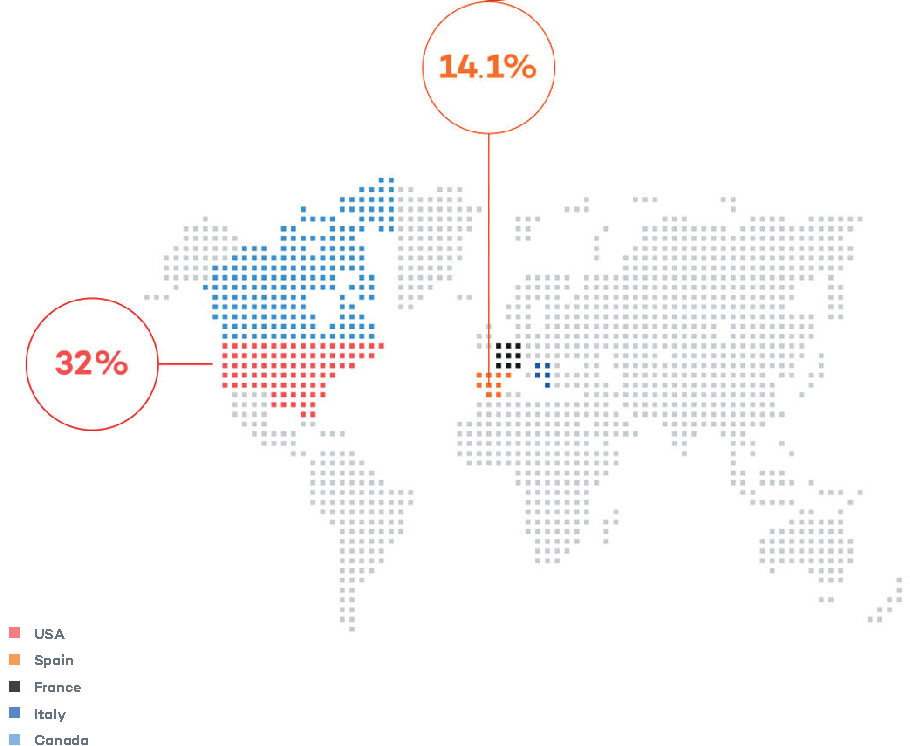
\includegraphics[width=13.5cm, keepaspectratio]{marco_teorico/pandasecurity_geography_cryptojacking.pdf}
    \caption*{\textbf{Fuente:} \cite{report:pandasecurity_coinhive_mining}}
  \end{figure}

  Este tipo de ataques se produce globalmente, desapareció casi totalmente a finales del año 2011 pero volvió a surgir a finales del año 2017, debido al hecho de que los navegadores web tienen más accesos al hardware como GPUs\footnote{Graphics Processing Unit (Unidad de Procesamiento de Gráficos)} y a funciones de criptografía específicas en la CPU.

  De acuerdo con \cite[p.~13]{report:pandasecurity_coinhive_mining}, el 59\% de las empresas en el Reino Unido han sido infectadas al menos por un gusano mediante este tipo de ataques.

  Según el reporte \cite[p.~22]{report:mcafee_threats} de Mcafee, el volumen de ataques de minería de criptomonedas se incrementó en 29\% en el primer trimestre del año 2019 ya que los objetivos ya no son solo los servidores web y de aplicaciones, sino también los clientes Windows, Linux, Apple, iOS y Android.

  \begin{figure}[ht]
    \centering
    \caption{Nuevas infecciones para minería de criptomonedas}
    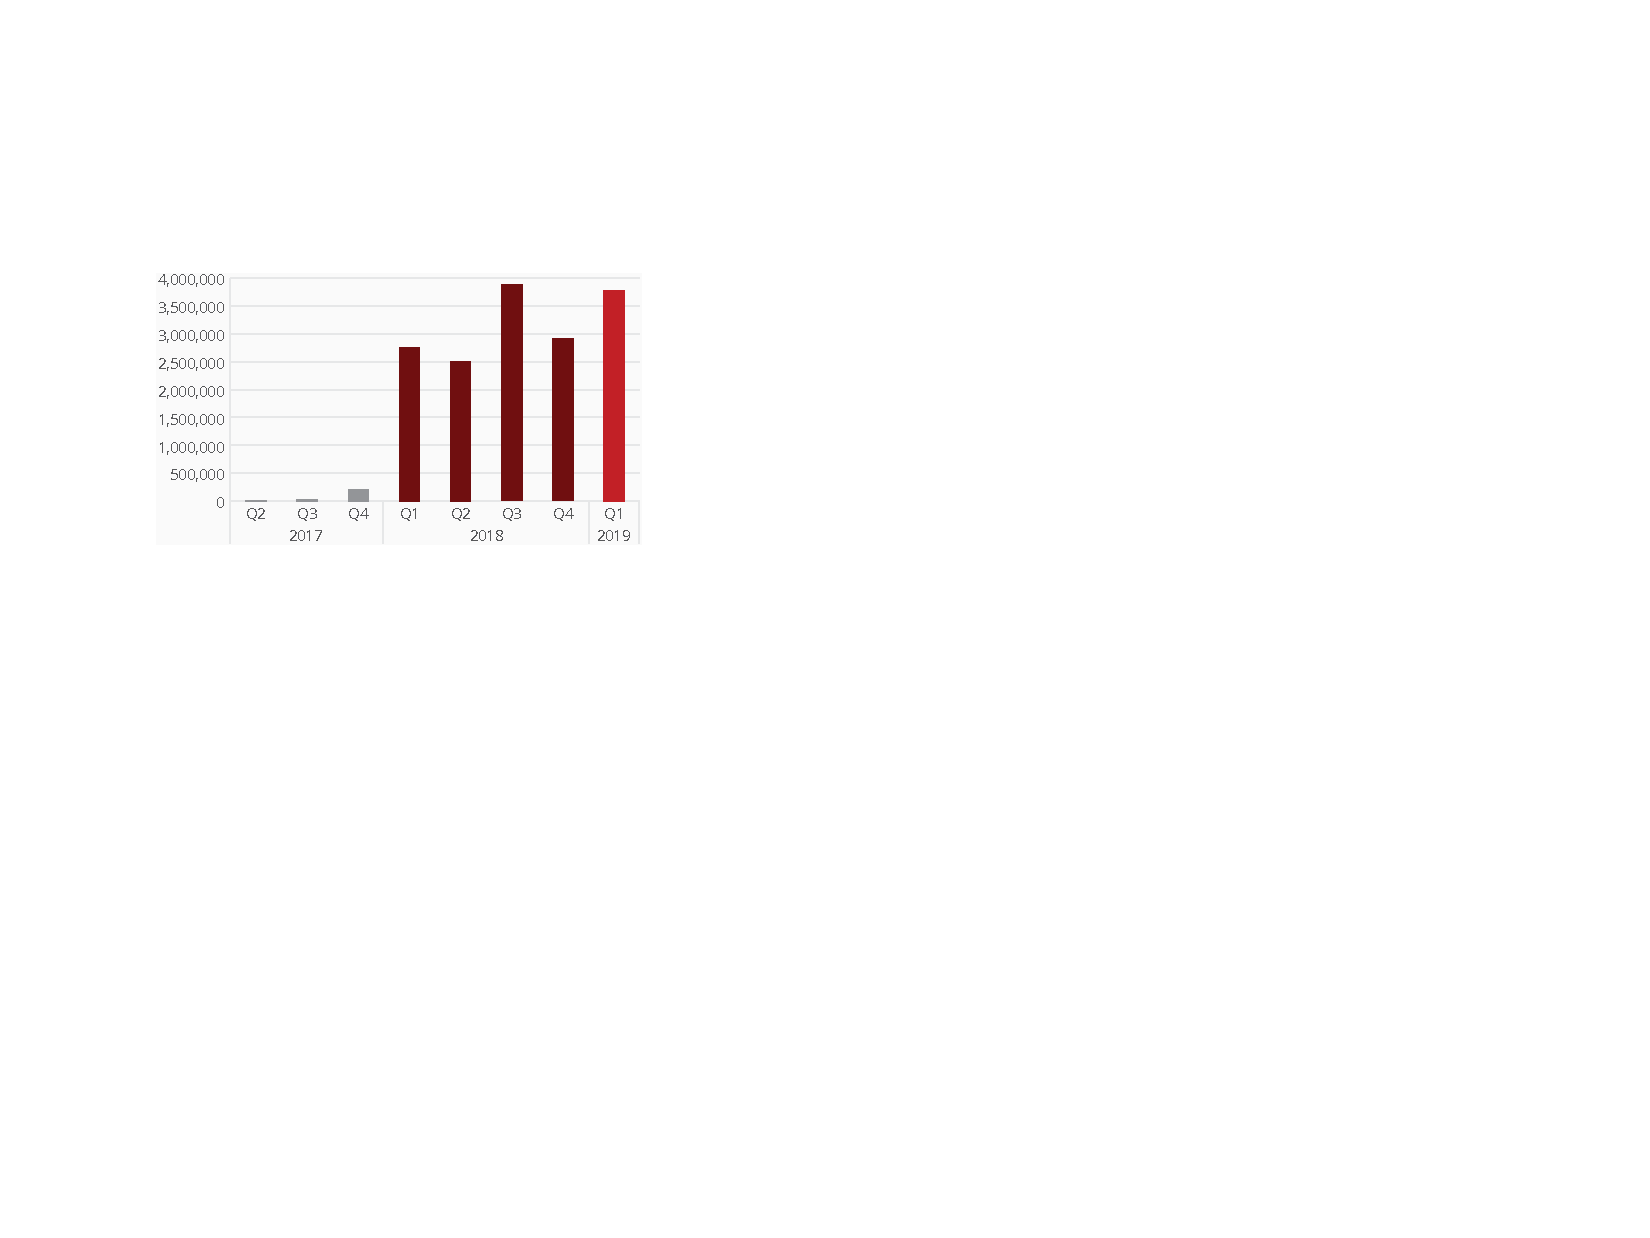
\includegraphics[width=12cm, keepaspectratio]{marco_teorico/mcafee_new_miner.pdf}
    \caption*{\textbf{Fuente:} \cite{report:mcafee_threats}}
  \end{figure}

  Este tipo de ataques ya no se producen de manera aislada o esporádica, por lo cual es necesario obtener la mayor información posible del proceso de infección y tomar en cuenta las recomendaciones para evitar infecciones por minería de criptomonedas.

  \section{Blockchain y criptomonedas}

  La definición de criptomoneda no es un concepto reciente, de hecho \cite{article:wei_dai_money}, publicó en su white paper los cinco pilares del protocolo en los que actualmente se basa la criptoeconomía:

  \begin{enumerate}
    \item Cualquier nodo en la red puede crear monedas transmitiendo la solución a un problema computacional previamente no resuelto. Las únicas condiciones son que debe ser fácil determinar cuánto esfuerzo informático tomó para resolver el problema y la solución no debe tener valor, ya sea práctico o intelectual. El número de unidades monetarias creadas es igual al costo del esfuerzo informático. A este concepto se le denominó minería posteriormente.
    \item Si un nodo desea transferir dinero a otro nodo, el primer nodo (Alicia) transmite el mensaje ``Doy X unidades de dinero a Bob'' firmado por Alicia. Sobre la transmisión de este mensaje, todos debitan la cuenta de Alicia por X unidades y acreditan a la cuenta Bob X unidades, a menos que esto cree un negativo
    saldo en la cuenta de Alicia en cuyo caso se ignora el mensaje.
    \item Un contrato válido debe incluir una garantía en caso de incumplimiento para cada parte participante del mismo. También incluye un árbitro en caso de que haya una disputa. Todas las partes en un contrato, incluido el árbitro, deben transmitir sus firmas antes de que entre en vigencia. Tras la emisión del contrato y todas las firmas, cada participante carga la cuenta de cada parte por el monto de la garantía máxima y se acredita también a un hash del contrato con la suma del máximo de indemnización. El contrato se hace efectivo si los débitos tienen éxito en cada parte sin producir un saldo negativo, de lo contrario el contrato se ignora y las cuentas se revierten
    \item Si un contrato concluye sin disputa, cada parte transmite un mensaje firmado ``El contrato con hash SHA-1 concluye sin ejecución de garantías. O posiblemente, el contrato con hash SHA-1 concluye con las siguientes garantías: ...''. Tras la emisión de todas las firmas, cada participante acredita la cuenta de cada parte por el monto de la garantía máxima, elimina la cuenta del contrato, luego acredita o debita la cuenta de cada parte de acuerdo con el cronograma de garantías, si lo hay.
    \item Si las partes de un contrato no pueden llegar a un acuerdo sobre una conclusión apropiada incluso con la ayuda del árbitro, cada parte difunde un calendario de garantías/multas sugerido y cualquier argumento o evidencia a su favor. Cada participante toma una determinación en cuanto a reparaciones reales y/o multas, y modifica sus cuentas en consecuencia.
  \end{enumerate}

  Cada período de creación de dinero se divide en cuatro fases:

  \begin{enumerate}
    \item Los titulares de las cuentas calculan y negocian entre sí para determinar un aumento óptimo en la oferta de dinero para el próximo período. Independientemente de si los titulares de cuentas pueden alcanzar un consenso, cada uno transmite su cuota de creación de dinero y cualquier cálculo macroeconómico realizado para respaldar las cifras.
    \item Cualquiera que quiera crear dinero emite una oferta en forma de $<x, y>$ donde $x$ es la cantidad de dinero que quiere crear, e $y$ es un problema no resuelto de una clase de problema predeterminada. Cada problema debe tener un costo nominal (en años MIPS\footnote{Millions of Instructions Per Second (Millones de Instrucciones Por Segundo)}, por ejemplo) que se acuerde públicamente.
    \item Después de ver las ofertas, los que presentaron ofertas en la fase de licitación ahora pueden resolver los problemas en sus ofertas y transmitir las soluciones.
    \item Cada administrador de cuentas acepta las ofertas más altas (entre las que realmente emitieron soluciones) en términos de costo nominal por unidad de dinero creado y acredita las cuentas de los licitantes en consecuencia.
  \end{enumerate}

  En base a estos preceptos Satoshi Nakamoto, personaje desconocido hasta la fecha, diseñó un sistema de dinero digital de código abierto llamado ``Bitcoin'', este sistema vió la luz el 9 de enero de 2009 con un cambio menor a 0,05\$us, llegando a su auge en diciembre de 2017 con un cambio de 17.549,67\$us. Al momento del presente análisis esta criptomoneda estuvo a un cambio de 8.704,04\$us, de acuerdo a los datos obtenidos de \cite{web:bitstamp}.

  \begin{figure}[H]
    \centering
    \caption{Precio histórico del Bitcoin}
    \newcommand\csvfile{../inc/marco_teorico/bitcoin_price.csv}
    \pgfplotstableread[col sep=comma]{\csvfile}\datatable
    \begin{tikzpicture}
      \begin{axis}[
        width=14cm,
        ymajorgrids=true,
        tick pos=left,
        xtick=data,
        xticklabels from table={\datatable}{YEAR},
        xticklabel style={font=\small, rotate=80, anchor=east},
        enlarge x limits=-0.1,
        enlarge y limits=-0.1,
        xlabel={Año},
        ylabel={Precio [\$us]},
        yticklabels={0,1000,2000,3000,4000,5000,6000,7000,8000,9000,10000,11000,12000,13000,14000,15000,16000,17000,18000},
        ytick={0,1000,2000,3000,4000,5000,6000,7000,8000,9000,10000,11000,12000,13000,14000,15000,16000,17000,18000},
        ytick scale label code/.code={},
        ymin=0,
        ymax=18000,
        tick style={draw=none}
      ]
        \addplot[blue, line width=1pt] table [x expr=\coordindex, y=PRICE, col sep=comma] {\csvfile};
      \end{axis}
    \end{tikzpicture}
    \caption*{\textbf{Fuente:} \cite{web:bitstamp}}
  \end{figure}

  La propuesta de Bitcoin conlleva también un registro de balance económico público basado en Blockchain\footnote{Cadena de Bloques}, esto significa que cada transacción lleva la firma digital representada por el hash de cada una de las partes del contrato, como se muestra en la Figura \ref{fig:bitcoin_transaction}.

  \begin{figure}[ht]
    \centering
    \caption{Transacción mediante Blockchain}
    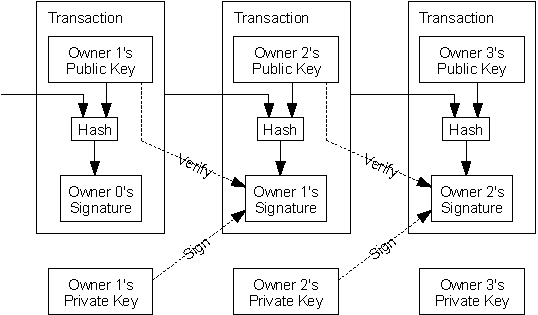
\includegraphics[width=12cm, keepaspectratio]{marco_teorico/bitcoin_transaction.pdf}
    \caption*{\textbf{Fuente:} \cite[p.~2]{article:satoshi_bitcoin}}
    \label{fig:bitcoin_transaction}
  \end{figure}

  Cada transacción puede ser resuelta por más de un nodo al mismo tiempo por lo cual, el nodo que demuestre el cómputo más económico tiene derecho a reclamar lo que se denomina espacio de disco, esto evita las ramas de hashes huérfanos y produce un nuevo Árbol de Merkle, como se muestra en la Figura \ref{fig:bitcoin_disk_space}, que prácticamente es un hash que se basa en toda la historia de transacciones aceptadas en quorum por la mayoría de los nodos, generando así un único registro histórico de transacciones, descentralizado y compartido por todos los nodos.

  \begin{figure}[ht]
    \centering
    \caption{Selección del cómputo más económico}
    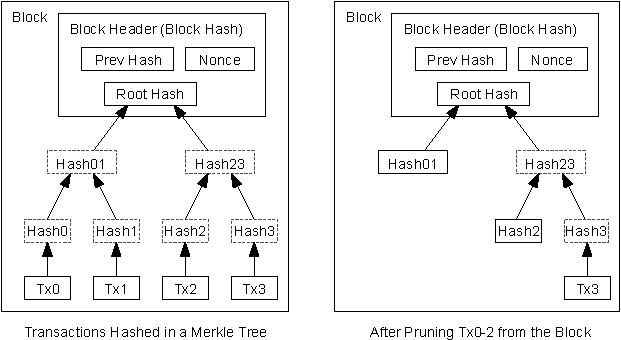
\includegraphics[width=12cm, keepaspectratio]{marco_teorico/bitcoin_disk_space.pdf}
    \caption*{\textbf{Fuente:} \cite[p.~4]{article:satoshi_bitcoin}}
    \label{fig:bitcoin_disk_space}
  \end{figure}






\end{document}
